\section*{TLB (faster translation)}
TLB performance (cache perf. in general) improved by two factors:
\begin{enumerate}
\item Spatial locality:  if a program accesses memory at address x , it
will likely soon access memory near x
\item Temporal locality:  ix recently accessed will likely be accessed soon
\end{enumerate}
\section*{TLB Control Flow Algorithm}
\begin{minipage}{.66\linewidth}
\begin{lstlisting}[language=c]
VPN = (VirtualAddr & VPN_MASK) >> SHIFT
(Success, TlbEntry) = TLB_Lookup(VPN)
if (Success == True) // TLB Hit
  if (CanAccess(TlbEntry.ProtectBits) == True)
    Offset = VirtualAddr & OFFSET_MASK
    PhysAddr = (TlbEntry.PFN << SHIFT) | Offset
    Register = AccessMemory(PhysAddr)
  else
    RaiseException(PROTECTION_FAULT)
else // TLB Miss
  PTEAddr = PTBR + (VPN * sizeof(PTE))
  PTE = AccessMemory(PTEAddr)
  if (PTE.Valid == False)
    RaiseException(SEGMENTATION_FAULT)
  else if (CanAccess(PTE.ProtectBits) == False)
    RaiseException(PROTECTION_FAULT)
  else
    TLB_Insert(VPN, PTE.PFN, PTE.ProtectBits)
    RetryInstruction()
\end{lstlisting}
\begin{lstlisting}[language=c]
VPN = (VirtualAddr & VPN_MASK) >> SHIFT
(Success, TlbEntry) = TLB_Lookup(VPN)
if (Success == True) // TLB Hit
  if (CanAccess(TlbEntry.ProtectBits) == True)
    Offset = VirtualAddr & OFFSET_MASK
    PhysAddr = (TlbEntry.PFN << SHIFT) | Offset
    Register = AccessMemory(PhysAddr)
  else
    RaiseException(PROTECTION_FAULT)
  else // TLB Miss
    RaiseException(TLB_MISS)
\end{lstlisting}
\end{minipage}
\begin{minipage}{.34\linewidth}
  \flushleft
  \begin{itemize}
  \item CISC TLB miss $\to$HW
    \begin{enumerate}
    \item page table register stored in memory
    \item walk page table, find correct PTE, extract translation
    \item update TLB with the translation
    \item retry the instruction
    \end{enumerate}
  \item RISC TLB miss $\to$OS
    \begin{enumerate}
    \item hardware raises exception$\to$pause
    \item kernel mode$\to$trap
    \item OS updates TLB; returns from trap
    \end{enumerate}
  \item accessing large num of pages, exceeding \textbf{TLB} \textbf{coverage} in a short time $\to$ lots TLB miss
  \item TLB can be \textbf{bottleneck} in CPU pipeline, esp. with physically-indexed cache, because addr trans has to happen \emph{before} cache is accessed

  \end{itemize}
\end{minipage}
\section*{TLB Control Flow Algorithm (OS Handled)}
\begin{itemize}
\item when returning from a TLB miss-handling trap, hardware must resume execution at the ix that caused the trap, resulting in a TLB hit
\item OS must not cause infinite chain of TLB misses to occur
  \begin{enumerate}
  \item keep TLB miss handlers in physical mem (unmapped, no addr trans)
  \item reserve entries in TLB for permanently-valid trans and handler code itself (these wired translations always TLB hit)
  \end{enumerate}
\end{itemize}
\section*{TLB Entries (hardware search all entries for a match)}
\begin{minipage}{.45\linewidth}
  \flushleft
  \begin{enumerate}
  \item typically small (32/64/128 entries)
  \item \textbf{not} indexed by VPN
  \item \textbf{fully associative}
  \end{enumerate}
\end{minipage}
\begin{minipage}{.55\linewidth}
  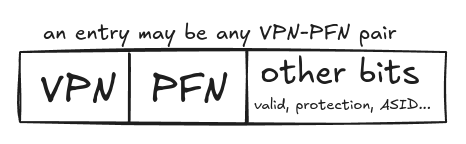
\includegraphics[width=\linewidth]{imgs/tlb_entry}
\end{minipage}
\section*{TLB: Context Switch}
\begin{minipage}{.45\linewidth}
  \flushleft
  \begin{enumerate}
  \item \textbf{flush} all entries
    \begin{itemize}
    \item whenever a proc resumes $\to$ TLB misses
    \item if ctx switch too frequently $to$ too costly
    \end{itemize}
  \end{enumerate}
\end{minipage}
\begin{minipage}{.55\linewidth}
  \begin{tabular}{ccccc}
    VPN & PFN & valid & prot & ASID \\
    \hline
    10 & 100  &   1   & rws  & 1    \\
    -  &  -   &   -   & -    & -    \\
    10 & 170  &   1   & rwx  & 2    \\
    \hline
  \end{tabular}
\end{minipage}
\begin{enumerate}
\item[2.] addr space identifier (ASID) to each TLB entry
  \begin{itemize}
  \item each proc with unique ASID
  \item entries contain different procs at same time while keep isolation
  \end{itemize}
\end{enumerate}
\section*{TLB: Replacement Policy (minimize miss rate or inc hit rate)}
\begin{enumerate}
\item replace \textbf{least-recently-used} (LRU)
\item evict a \textbf{random} entry
\end{enumerate}
